\section{Problem Formulation}
Given an image $X$ and a query object of class $c_q$ ($q \in {1,..,C}$), we detect
the query object by sequentially choosing one
context class to detect, and narrow down the search area for the query object based on
observed detector responses. 
The sequential decision-making problem can be formulated as a Markov Decision
Process (MDP).
\begin{mydef}
The \textbf{Object Detection MDP} is defined by the tuple $(\mathcal{S}, \mathcal{A}, T(.), R(.), \gamma)$:
\begin{itemize}
\item The \textbf{state} $s_t=(X^t, O^t)$, where $X^t$ is the search area for the
query at time $t$ (initially $X^0$ is the entire image $X$), $O^t= \{o_1, o_2,
\dots, o_t\}$ is a sequence of observed responses from applied contextual
classifiers;
\item The \textbf{action} set $\mathcal{A} = \{a_1, \dots, a_C, Stop,
Reject\}$, where $a_i$ corresponds to running the detector of class
$c_i$, \textit{Reject} means to reject the query class as occurring in the
image and terminate the process, and \textit{Stop} outputs the search area
and run the detector of the query class;
\item The \textbf{state transition} function $T(s'|s,a)$ defines a
next-state distribution after action $a$ is taken in state $s$, which is deterministic in our case;
\item The \textbf{reward} function $R(s,a) \rightarrow \mathbb{R}$ evaluates
how good it is to take action $a$ in state $s$;
\item The \textbf{discount} factor $\gamma$ is a constant controlling
the tradeoff between greedily maximizing the immediate
reward and the long term expected reward.
\end{itemize}
\end{mydef}

We define the \textit{reward} $R$ as the immediate gain in an intersection/union model of the search space:
\begin{eqnarray}
\label{eq:imreward}
R(s_t,a_t) =  \frac{X^{t+1} \cap X_q}{X^{t+1} \cup X_q} - \frac{X^{t}\cap X_q}{X^{t} \cup X_q}
\end{eqnarray}
where $X^{t+1}$ is the updated search area after executing action $a_t$ in state $s_t$, determined by the context models described in Section~\ref{sec:context}. $X_q$ is the groundtruth mask of the query object instances in the image. 

The query agent follows a
\textit{policy} $\pi: S \rightarrow A$ that determines which action to take in a
given state. 
Given an optimal policy $\pi^\ast$ which yields a state-action sequence that maximizes the discounted cumulative reward,
the optimal $Q$-value is recursively defined as $Q^\ast(s_t, a_t) = R(s_t, a_t) + \gamma\max_{a_{t+1}}Q^\ast(s_{t+1}, a_{t+1})$, where $a_t$ is chosen by $\pi^\ast$ and $\gamma$ is the discount factor.
Our goal is to learn the optimal policy for the object detection MDP.

\section{Approach}
We show our framework in Figure~\ref{fig:flowchart}.
Given a query, we first generate region hypotheses using object proposal algorithms, 
then the policy sequentially selects an action that rejects the occurrence of the query, poses a question about a context class, or stop and run the query detector. 
After an action is taken, the search locations are updated based on the responses and
new posterior probabilities of each category are computed to update the state.
In this section, we first present the imitation learning algorithm for learning a policy that plays the twenty questions game; 
we then describe how to refine the search area of the query given responses of contextual classifiers evaluated by previous questions.

\subsection{Learning the Policy by Imitation}
Typically, MDPs are solved by reinforcement learning (e.g., Q-learning~\cite{watkins1992q},
REINFORCE~\cite{williams1992simple}). However, given our exponential search space, such trial-and-error
approaches can take long to converge.
We therefore take the imitation learning approach, where we assume direct supervising
signals from the oracle are available and learn to mimic the oracle's
behavior.

Assuming we know the optimal $Q$-values, the optimal policy is
straightforward 
\begin{eqnarray}
\label{eq:pi}
\pi^\ast(s) = \arg\max_{a\in A} Q^\ast(s,a).
\end{eqnarray}
To learn $Q^\ast$, we assume these values are given
by an \emph{oracle} at training time; thus the
problem can be reduced to learning
a linear approximation:
\begin{eqnarray}
\label{eq:qvalue}
Q^{\ast}(s,a) = \theta_\pi^T \phi(s,a),
\end{eqnarray}
where $\phi(s,a) = \phi((X^t, O^t),a)$ is the state feature representing the search area $X^t$ and observations $O^t$ after observing detector responses of $a_1,...,a_t$. 
This can be solved by standard supervised learning approaches.

We compute the oracle's action sequence by breadth-first
search with pruning. The action sequence that maximizes the discounted
cumulative reward in the terminal state is selected as the oracle's action
sequence.
We then collect examples $\{(s_t,a_t,r_t)\}$ from the oracle's trajectory for
policy training.
However, collecting examples from the oracle's trajectory
only may result in mismatch in distributions of training and test data, since
the learned policy may go to state the oracle never visited.
To solve the mismatch problem, we encourage exploration by search multiple
times with random starting state.  Due to the large number of negative states for rejection, we sample the negative states by early pruning at negative immediate reward which imitates the early rejection action. After example collection, we train the policy (predict the optimal Q-values) by
ridge regression.

\begin{figure*}[htb]
\begin{center}
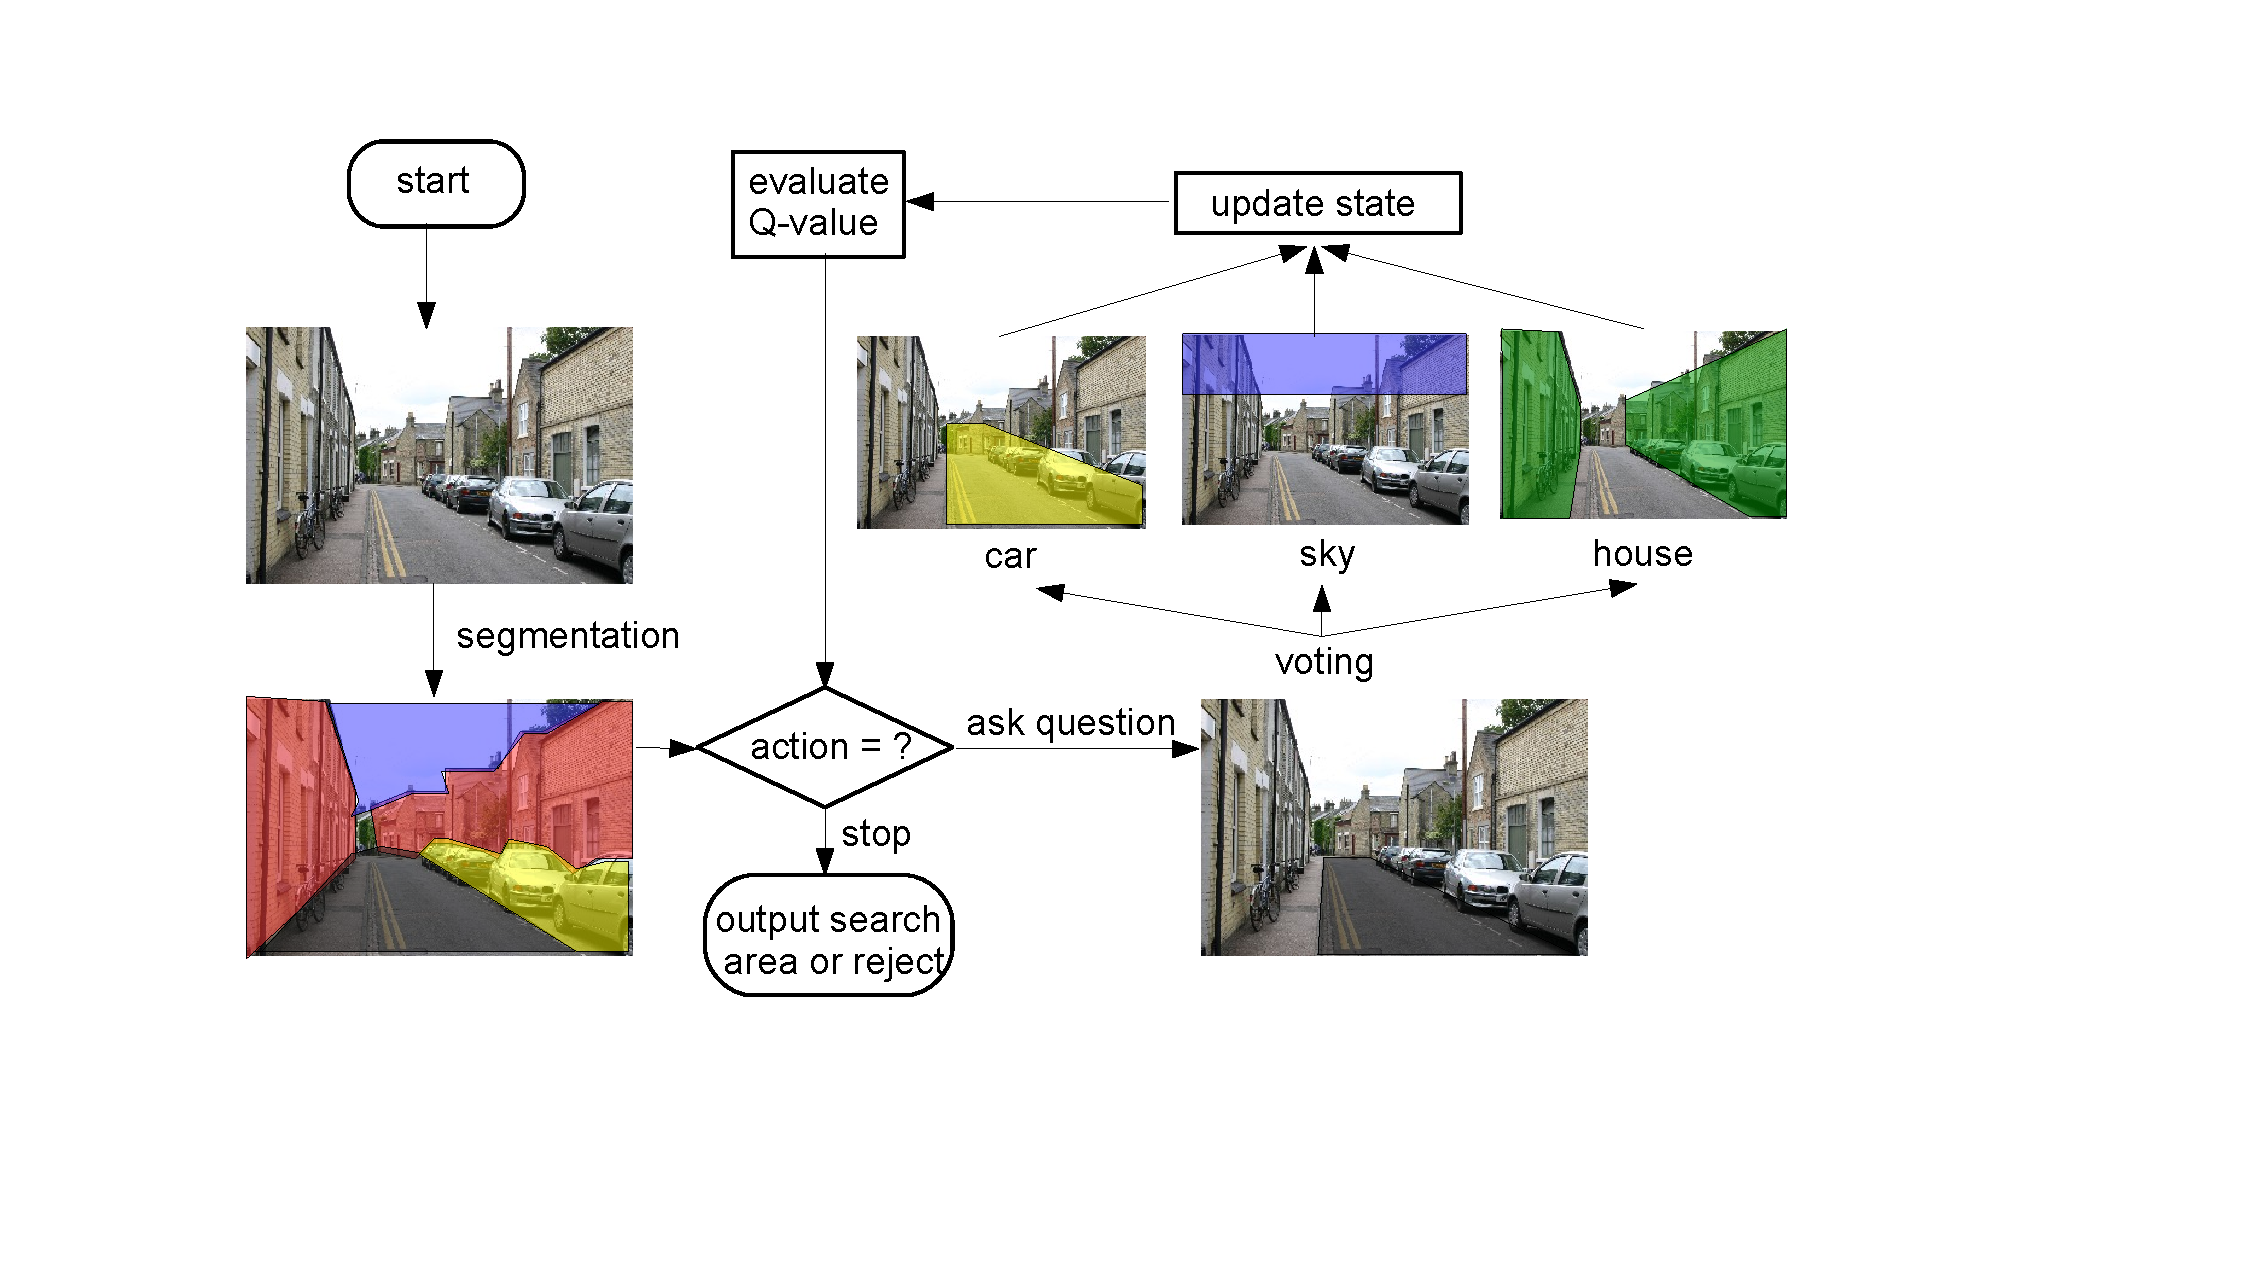
\includegraphics[width=0.8\linewidth]{figures/flowchart_Q.pdf}
\caption{Flowchart of our context driven object searching. %We first generate region hypotheses using object proposal algorithms, then the policy evaluates the current state and iteratively selects the action maximizing the Q-value function. Afterwards, the possible search locations are updated and the posterior probabilities of each category are evaluated for the next state.
}
\label{fig:flowchart}
\end{center}
\end{figure*}

\subsection{Context Modeling}
\label{sec:context}
Since our task is not only to detect instances of the query object but also to refine the search space of the query in the image as accurately as possible, conventional modeling of context as simple co-occurrence statistics is inadequate. Instead we present a data-driven location-aware approach to represent the spatial correlation between the objects and the scene. 

We capture the 

Given an action $a_t$ to detect context class $c_t$ at time $t$, we define $X_c \subset X$ as the \textit{exploration area for context} which excludes the observed regions of other contextual classes from the image. Here we formulate the context $p(c|c_t,X)$ as a posterior of the probabilistic vote map $p(c_t|c,X_c)$ defined on each pixel $(x_i,x_j)\in X$ over the image, and the responses of class $c_t$ after action $a_t$:
\begin{eqnarray}
p(c_t|c,X) = \sum_{X_c \subset X} p(c|c_t,X_c)p(c_t|X_c)
\end{eqnarray}

Given a refined search space $X_c\in X$ of a context class $c_t$ at time $t$, we formalize $p(c|c_t,X)$ as a weighted vote from the cooccurring region pairs of class $c_t$ and $c$ in training scenes. Let $(s_{c_t}^i, s_c^i)$ be the $i$-th pair of co-occurring regions of class $c_t$ and $c$, and $b_{c_t}^i$ and $b_c^i$ be their corresponding bounding boxes. We can now define the probabilistic vote map $p(c|c_t,X)$ as:
\begin{eqnarray}
\label{eq:votemap}
p(c|c_t,X_c) = \frac{1}{Z_c}\sum_i W(s_{c_t}^i,s;\theta^W).T(b_{c_t}^i,b_c^i)
\end{eqnarray}
where $s\in X^t$ is a region within the search space of the context class $c_t$. $Z_c$ is the normalization function. $W(.)$ is a kernel measuring similarity of region $s$ with a training region $s_i$. $T(b_{c_t}^i,b_c^i)$ models the transformation from $b_{c_t}^i$ to $b_c^i$, including translation and scaling. Figure~\ref{fig:votemap} shows a few examples of the vote maps. We can see that with the exemplar based and semantically aware voting, the resulting vote maps give more accurate search areas for the query objects.

% \begin{figure*}[t!]
%     \centering
%     \begin{subfigure}[b]{0.5\linewidth}
%         \centering
%         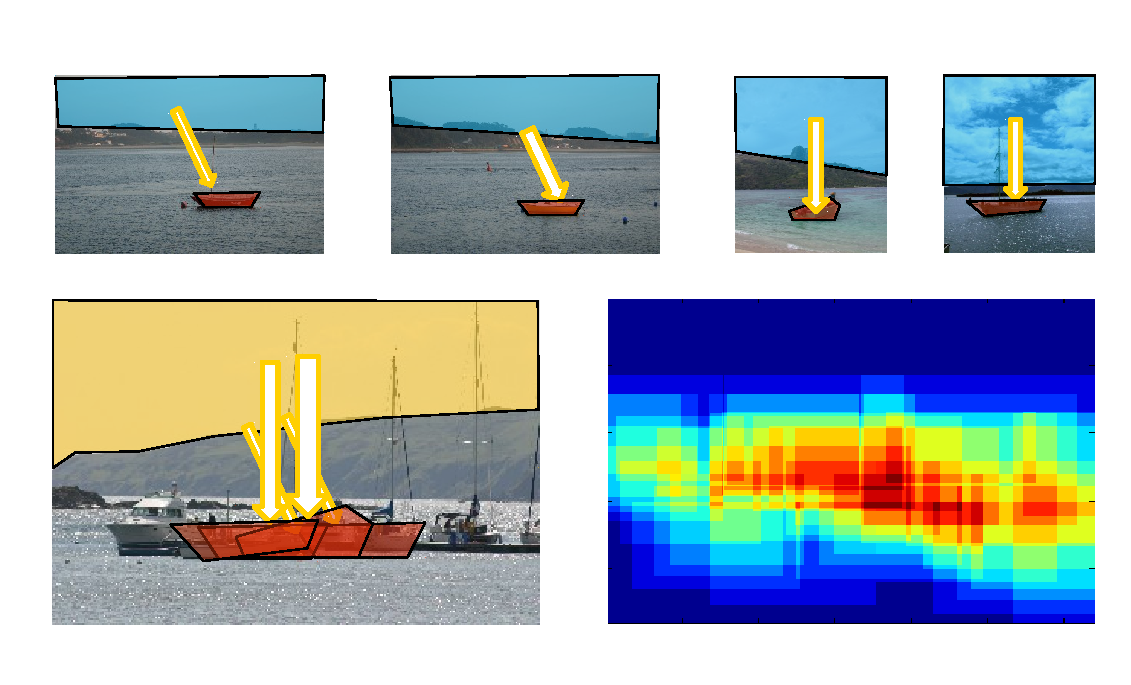
\includegraphics[width=0.5\linewidth]{figures/vote_sky_boat.pdf}
%         \caption{Lorem ipsum}
%     \end{subfigure}%
%     ~ 
%     \begin{subfigure}[b]{0.5\linewidth}
%         \centering
%         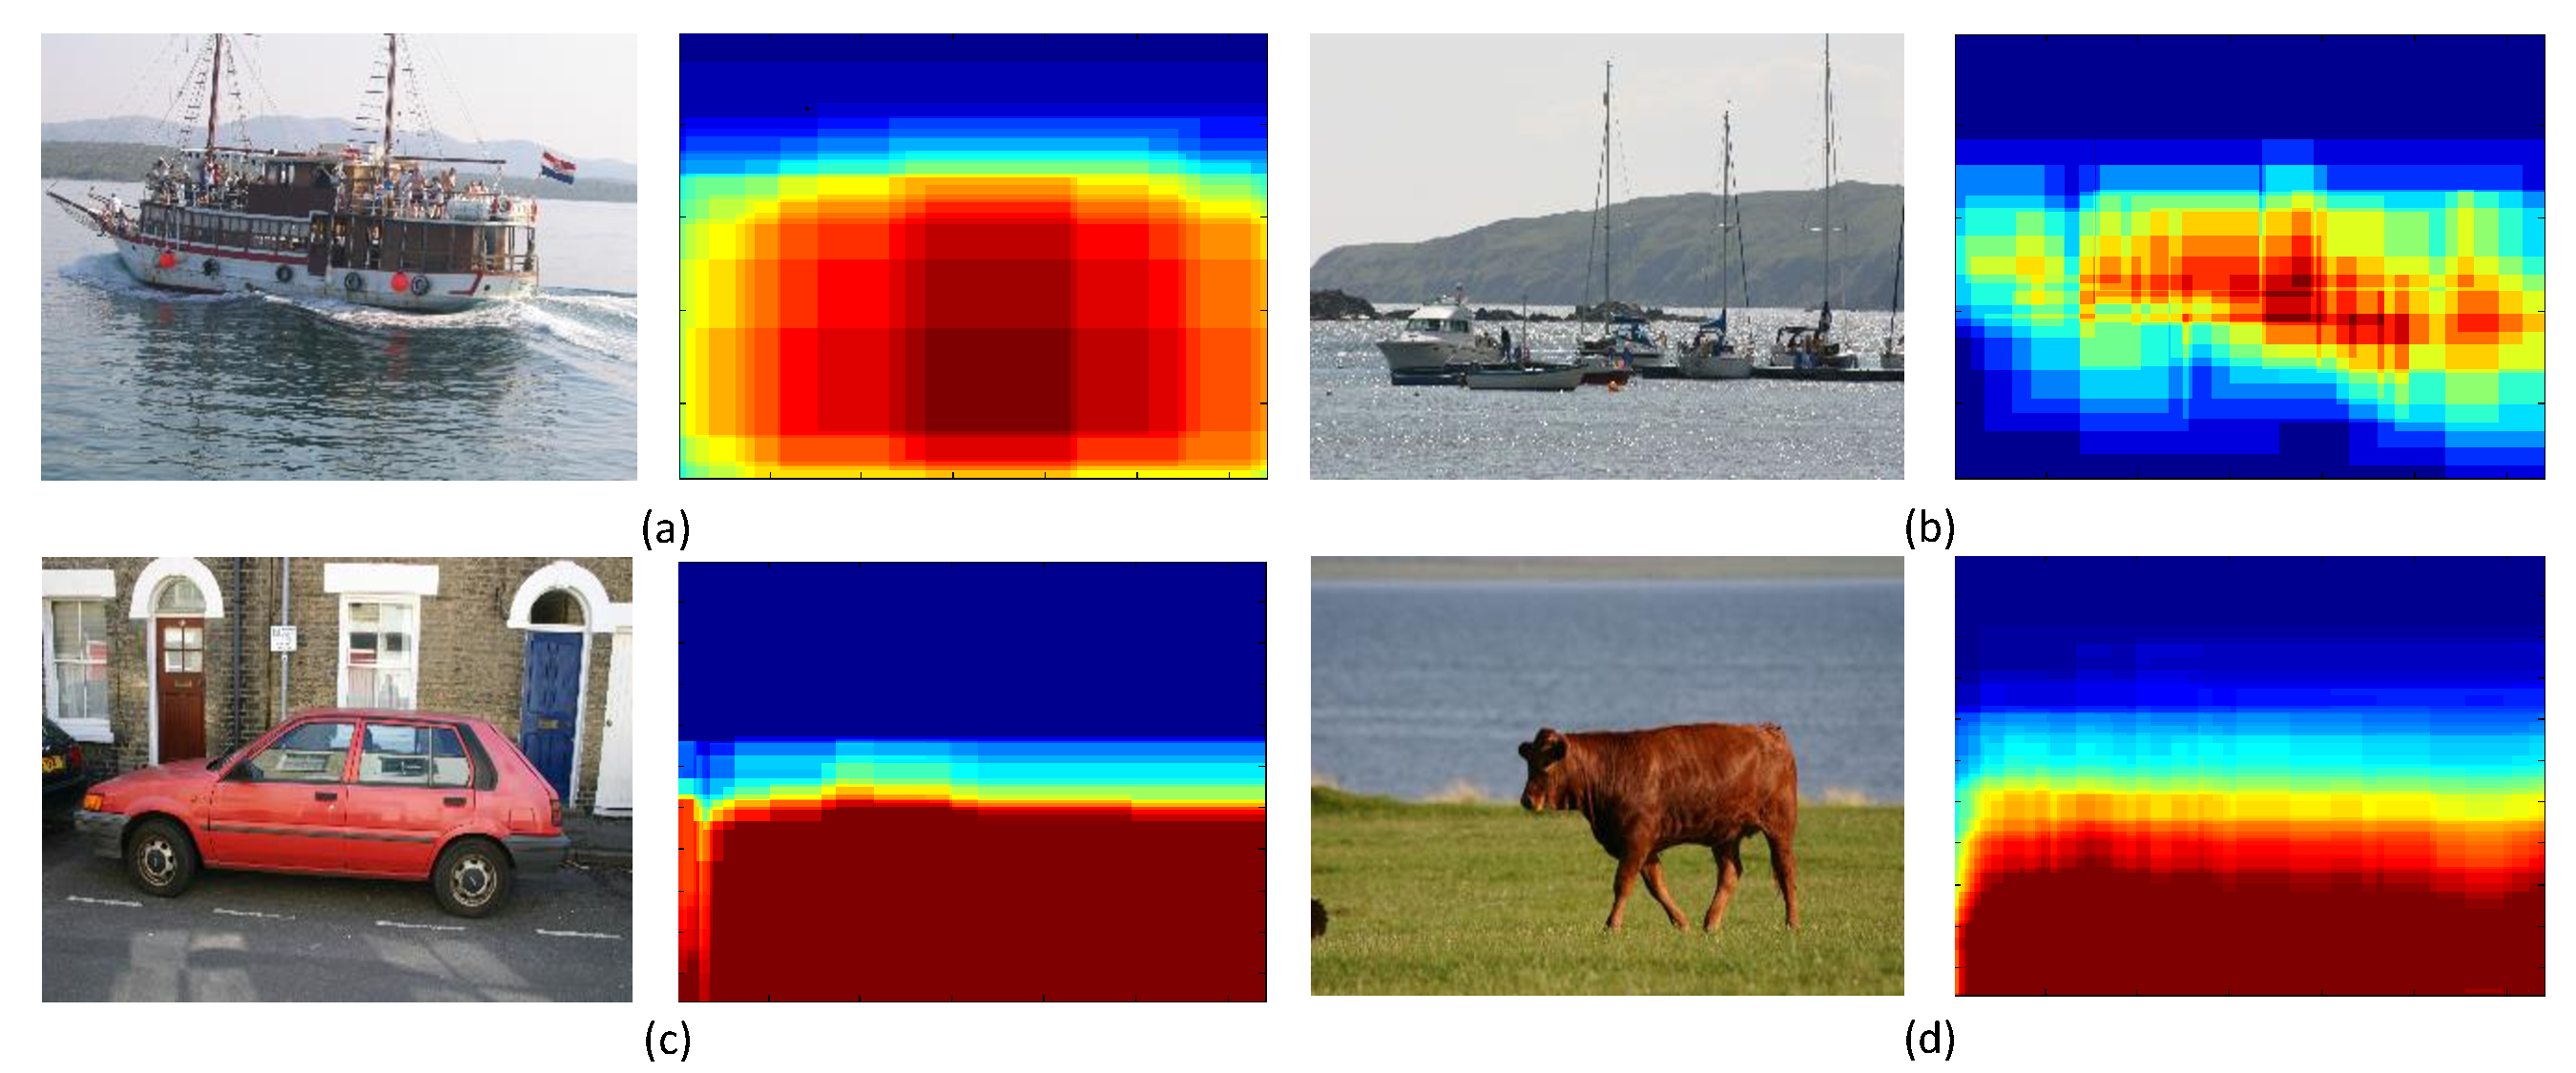
\includegraphics[width=0.5\linewidth]{figures/votemap.pdf}
%         \caption{Lorem ipsum, lorem ipsum,Lorem ipsum, lorem ipsum,Lorem ipsum}
%     \end{subfigure}
%     \caption{Caption place holder}
% \end{figure*}

% \begin{figure}[h]
% \centering
%  \subfloat[Subfigure 1 list of figures text][Subfigure 1 caption]{
% 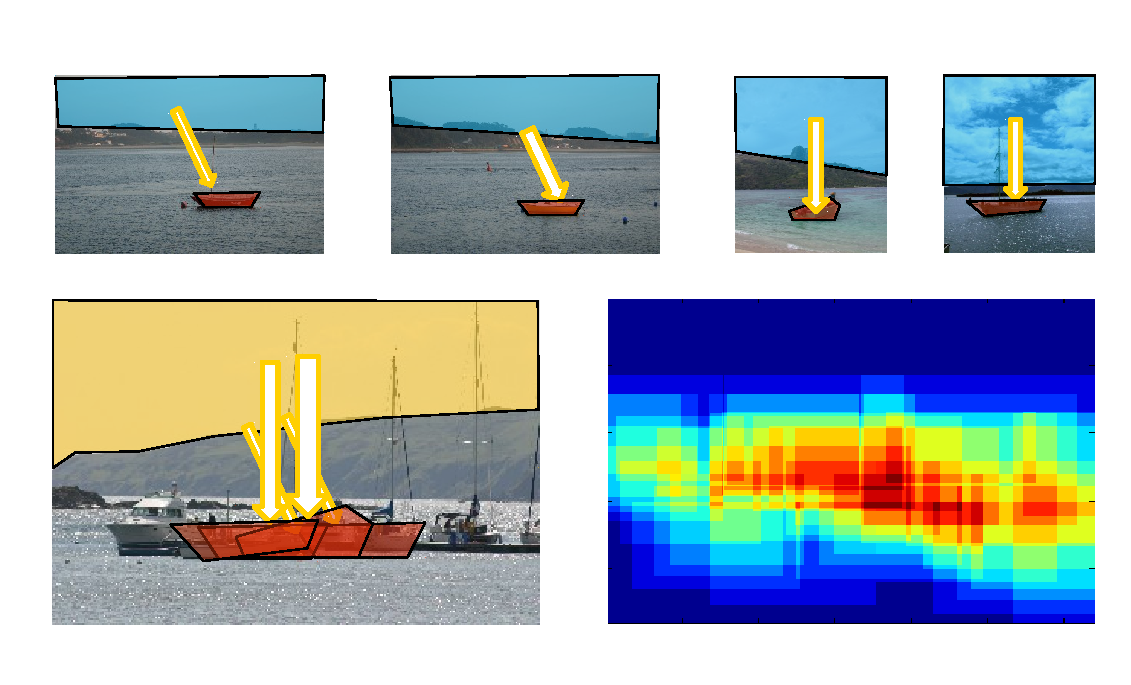
\includegraphics[width=0.4\textwidth]{figures/vote_sky_boat.pdf}
%  }
%  \subfloat[Subfigure 1 list of figures text][Subfigure 1 caption]{
% 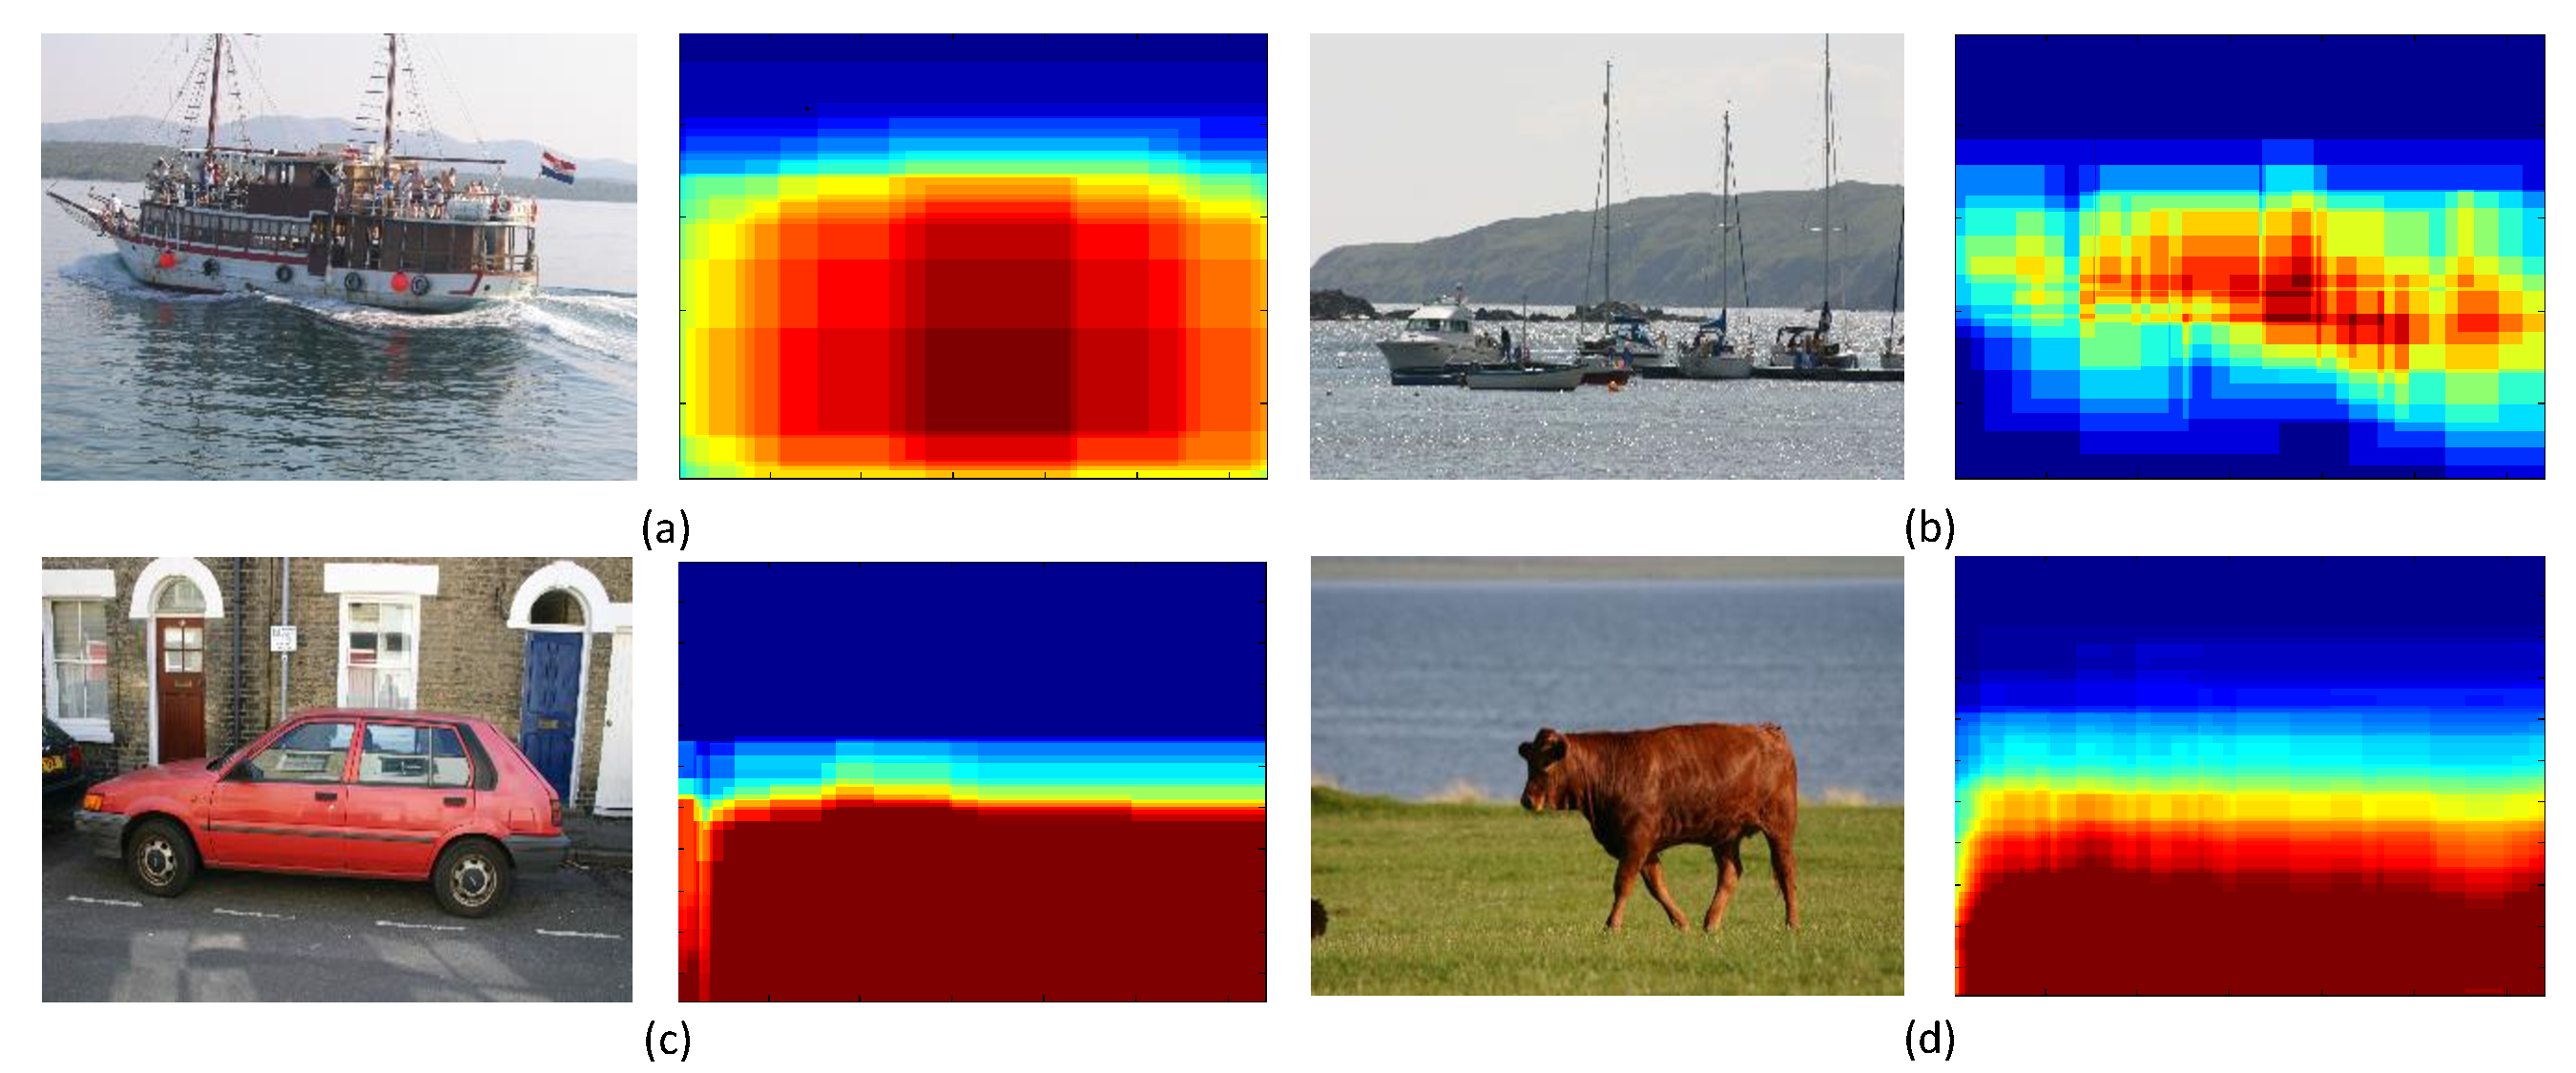
\includegraphics[width=0.4\textwidth]{figures/votemap.pdf}
%  }
% \end{figure}

\begin{figure}[ht!]
\begin{center}
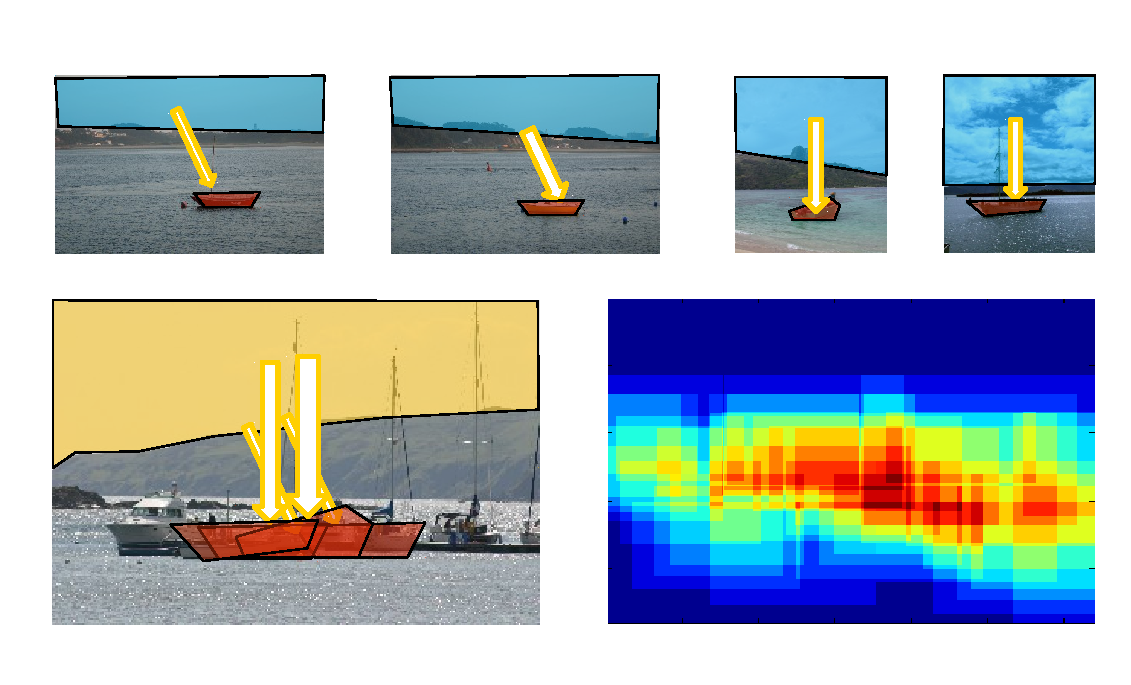
\includegraphics[width=0.6\linewidth]{figures/vote_sky_boat.pdf}
\end{center}
\caption{Examples of our weighted vote map for the context from sky to boat. The first rows are the training sample pairs of sky and boat and the second row is the test image and the resulted weighted voting map. The widths of the arrows denote the weighted similarity $W(s_{c_t}^i,s;\theta^W)$ between the test segment of sky (highlighted in yellow) and a training instance of sky segment (in light blue)}
\label{fig:vote_sky_boat}
\end{figure}


\begin{figure}[ht!]
\begin{center}
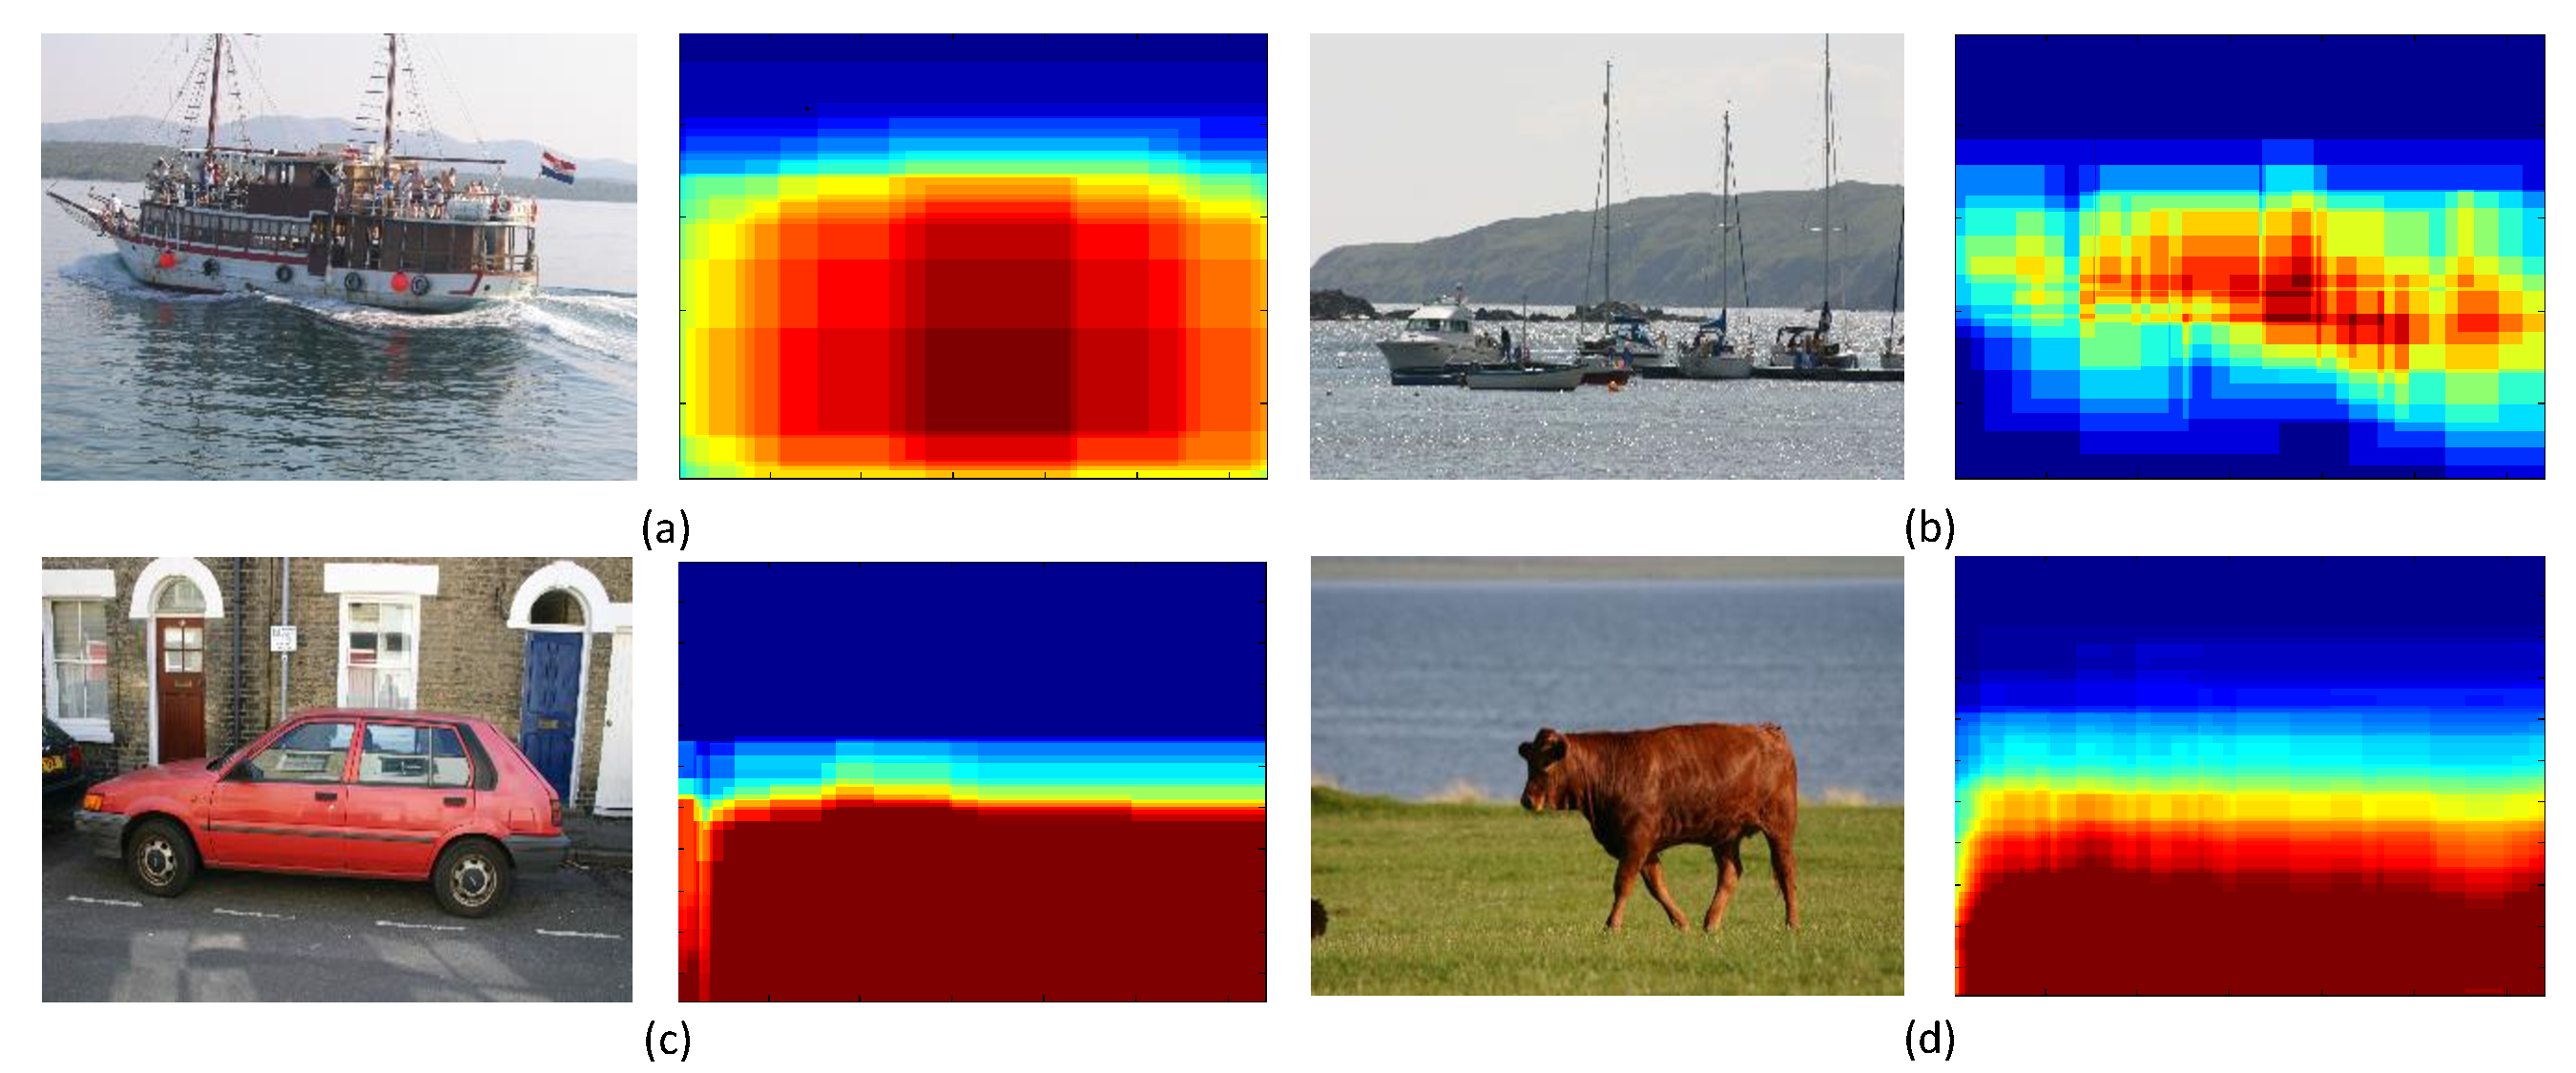
\includegraphics[width=0.6\linewidth]{figures/votemap.pdf}
\end{center}
\caption{Examples of our context vote maps. Each pair of images corresponds to the original image and the vote-based probability map of object location from observed context. From (a) - (d) are the vote maps from water to boat, sky to boat, road to car and grass to cow, respectively. Best viewed in color.}
\label{fig:votemap}
\end{figure}



The final context probabilistic vote map is given by
\begin{eqnarray}
p(c_t|c,X) = \sum_{s\in X_c} p(c_t|X_c)\sum_i W(s_{c_t}^i,s;\theta^W).T(b_{c_t}^i,b_c^i)\nonumber\\
\end{eqnarray}
where $p(c_t|X_c)$ is the probabilities of $s$ as class $c_t$ after taking the action $a_t$ to run classification at time $t$.


\subsection{Update Responses and Search Area}
After taking action $a_t$ and receiving response $o_t = p(c_t|c, X)$ from context class $c_t$, we integrate the response into observations from previous sequence of actions. Assuming the detectors and context classifiers are trained independently per category, the aggregated responses can be modeled as:
\begin{eqnarray}
p(O^t|c, X) = \prod_t p(c_t|c,X)
\end{eqnarray}

We then update the search area for the query class $c_q$ in a probabilistic framework:
\begin{eqnarray}
p(c_q|X,O^t) = \frac{p(O^t|c_q,X)p(c_q|X)}{Z}
\end{eqnarray}
where $Z = \sum_c^{C^t} p(O^t|c,X)p(c|X)$ is the partition function, $p(c|X)$ is obtained by taking actions and running context classifiers over the context segments,  and $C^t = \{c_1, c_2, ..., c_t, c_q\}$ are the set of observed contextual classes.
